% Este archivo es parte de la memoria del proyecto fin de carrera
% de Aarón Bueno Villares. Protegida bajo la licencia GFDL.
%
% Para más información, la licencia completa viene incluida en el
% fichero fdl-1.3.tex

% Copyright (C) 2010 Aarón Bueno Villares

\chapter{Manual de usuario}
\phantomsection
\label{manual}

En este manual se explica como jugar al videojuego
\gomf. En \gom usted compite, usando un ejército, contra el
ejército enemigo, ambos con pretensiones de ganar en el
enfrentamiento.

\section*{Menú principal del juego}
Al lanzar \gomf, lo primero con lo que nos encontramos es con
un menú con una ristra de 5 opciones:

\begin{itemize}
\item \textsc{Nueva batalla}
\item \textsc{Crear ejército}
\item \textsc{Editar ejército}
\item \textsc{Salir}
\end{itemize}

\begin{figure}[h]
\centering
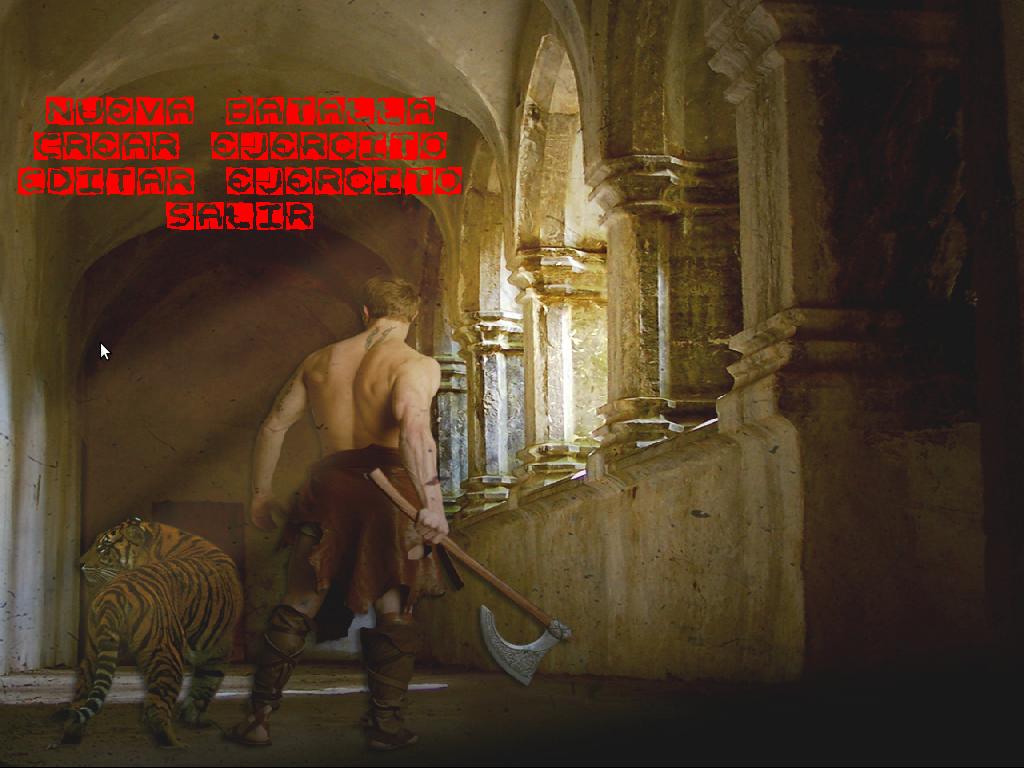
\includegraphics[scale=.4]{./imagenes/menuprincipal.png}
\label{fig:menuprincipal}
\caption{Menú principal del juego}
\end{figure}

\subsection*{\textsc{Nueva batalla}}
Al pulsar esta opción, se nos presenta un nuevo menú contextual para
elegir los ejércitos que protagonizarán la batalla. Se deberá escoger
al primer ejército, eligiendo un ejército de la lista de ejércitos
presente en el sumario, y pulsando la flecha que apunta a la primera
caja de texto, y al segundo ejército haciendo lo propio para la
segunda.

\begin{figure}[h]
\centering
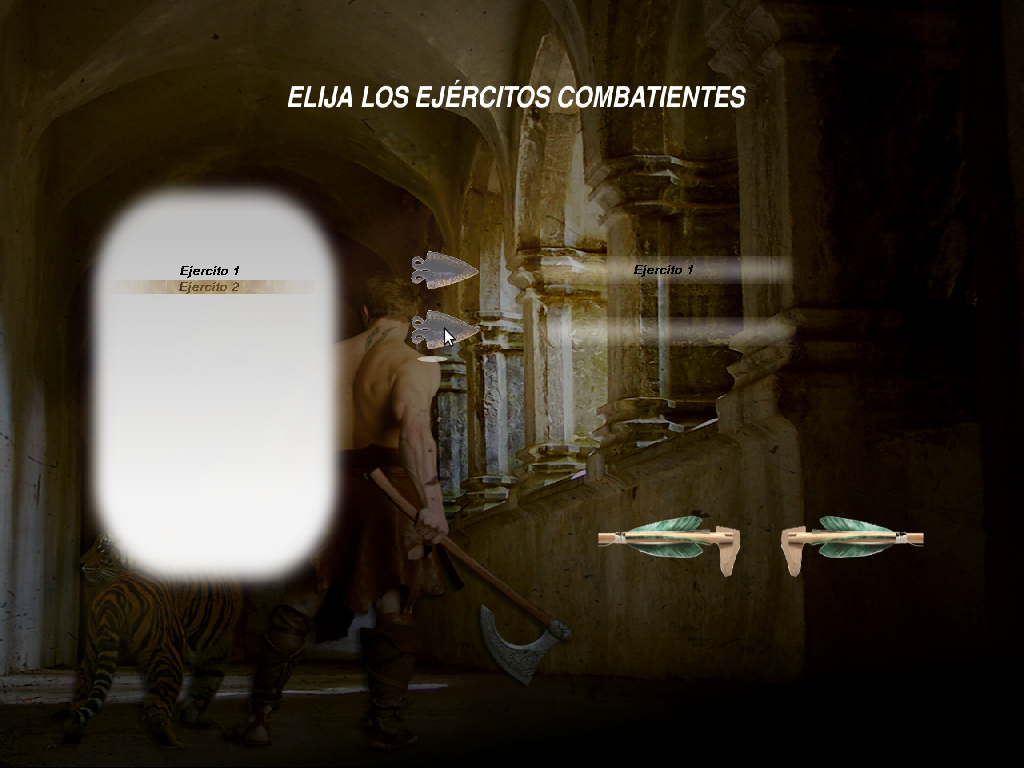
\includegraphics[scale=.4]{./imagenes/comenzarcombate.png}
\label{fig:comenzarcombate}
\caption{Menú de comienzo de batalla}
\end{figure}

Una vez elegidos ambos ejércitos, pulsamos la flecha que apunta a la
derecha, en la zona inferior de la pantalla, para comenzar una nueva
batalla, y se nos presenta el
escenario, con las unidades de ambos ejércitos desplegados, listo para
comenzar una batalla.

Si en vez de ir a la batalla, se desea cancelar la acción, basta
pulsar la flecha que apunta a la izquierda, en la zona inferior de la
pantalla, para regresar al menú principal.

\subsection*{\textsc{Crear ejército}}
En esta opción, se nos presenta una interfaz rica para editar nuestro
ejército con todas las herramientas necesarias para conseguirlo. Una
vez elegido un ejército, al pulsar a la flecha inferior que apunta a
la derecha, aparece una caja de texto para elegir el nombre de nuestro
ejército.

Este nombre puede estar formado por números, letras, barras bajas
(carácter '\_') y
espacios, pero no se pueden escribir ninguna otra clase de
carácteres. Una vez escrito, se vuelve a pulsar en la flecha derecha y
el ejército será añadido al sistema, y se volverá al menú
principal. Si se desea cancelar, se pulsa a la flecha izquierda y se
vuelve al menú de edición de ejércitos, con la misma configuración que
anteriormente. Ahora, si así lo deseas, puedes modificar tu ejército y
finalmente guardarlo.

Si al contrario, se desea cancelar la creación de un ejército, se
puede pulsar la flecha que apunta a la izquierda para retornar al menú
principal del juego.

\subsection*{\textsc{Editar ejército}}
Con esta opción, si se elige una unidad y se pulsa en la flecha
derecha, se llega al menú presentado en la sección anterior, salvo que
ahora se muestra en pantalla la configuración actual del ejército
elegido para la edición.

Se prosigue con en el caso anterior. Si se continúa, se puede
modificar el nombre del ejército, y luego añadir el nuevo nombre al
sistema.

\begin{figure}[h]
\centering
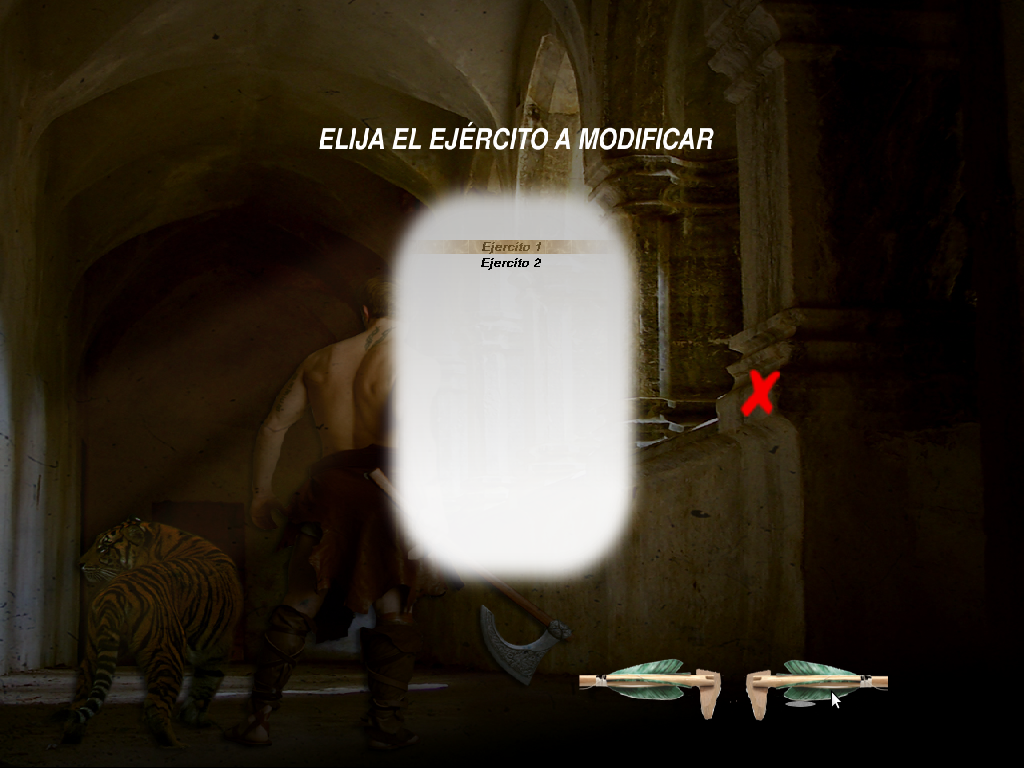
\includegraphics[scale=.4]{./imagenes/elegirejercito.png}
\label{fig:elegirejercito}
\caption{Menú de elección de ejército de edición}
\end{figure}

Con la flecha izquierda, se puede
retornar a pantallas anteriores sin deshacer los cambios.

Con la cruz roja se pueden eliminar ejército existentes, con solo
seleccionar el ejército y pulsar a continuación en la cruz roja.

\subsection*{\textsc{Salir}}
Con esta opción se abandona \gom y se cierra el programa.

\section*{Menú de edición de ejército}
Aquí se explica mas concisamente los elementos involucrados en el menú
de edición de un ejército.

Se pueden observar concretamente 5 secciones:
\begin{itemize}
\item El menú desplegable de elección de raza, en la parte
  superior izquierda de la pantalla.
\item La lista de unidades de raza, justo debajo del menú desplegable
  de elección de raza.
\item El sumario del ejército, en la parte medio e inferior derecha de
  la pantalla.
\item Los campos de edición de unidad, justo encima del sumario de
  unidades.
\item Las flechas de abandono y salvado del ejército, en la parte inferior
  derecha de la pantalla.
\end{itemize}

\begin{figure}[h]
\centering
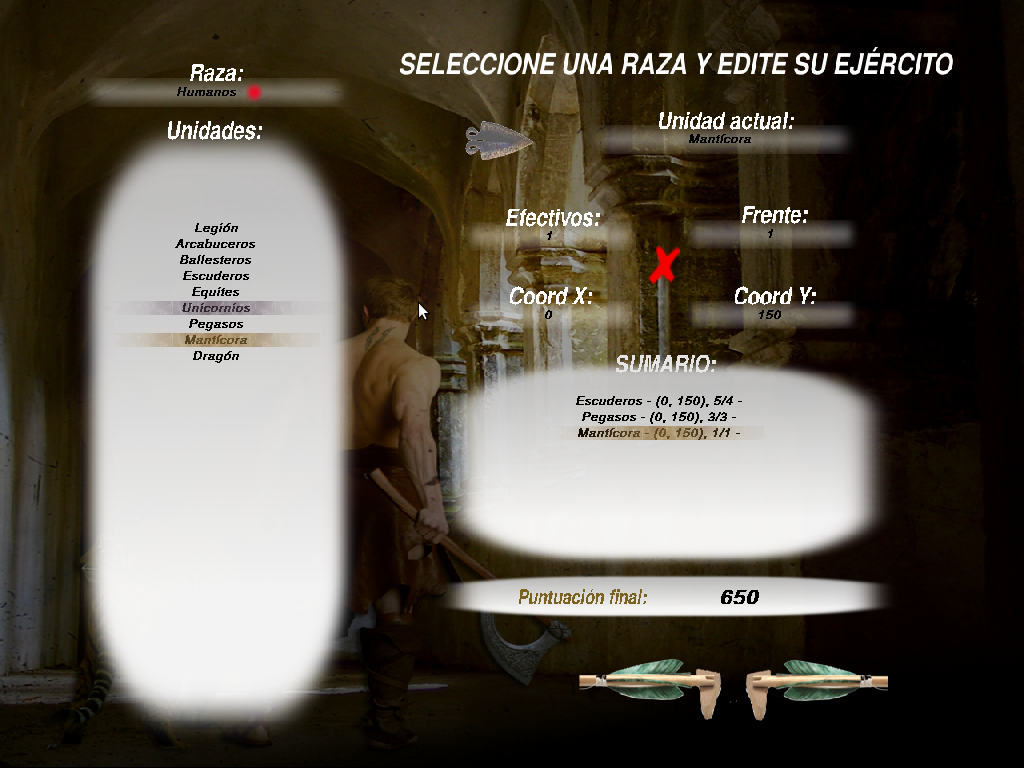
\includegraphics[scale=.4]{./imagenes/configurarejercito.png}
\label{fig:confejercito}
\caption{Menú de edición de ejército}
\end{figure}

\subsection*{Menú desplegable de elección de raza}
Es el recuadro titulado con el nombre \textsc{\textit{``Raza''}}. Si
se coloca el ratón encima del botón rojo, ese se ilumina, y si se
pulsa se despliega un menú en donde se puede elegir la raza de tu
ejército.

Una vez elegido, en la lista de unidades se muestran todas las
unidades disponibles para la raza elegida, que podrán seleccionarse
para añadirlas al sumario del ejército.

Si ya existía un ejército configurado, al cambiar de raza, toda la
información de la edición del ejército se borrará. Si se pulsa la
flecha de abandono, no se grabarán los cambios, y el ejército, si
existía, mantendrá su configuración original antes de la edición.

\subsubsection*{Lista de unidades de raza}
En esta lista se muestran todas las unidades disponibles para el
ejército elegido actualmente. Si se selecciona una unidad y se pulsa
la flecha situada mas arriba, esta unidad se añadirá al sumario de
unidades, y aparecerán los valores por defecto de la unidad en los
campos de edición de unidades, que podrán ser modificador inmediatamente.

Una vez pulsada una unidad, se podrán añadir tantas veces como se
desee con solo pulsar repetidas veces dicha flecha, con lo cual se
enriquecerá el sumario y aumentará el tamaño en puntos y el número de
unidades de tu ejército.

\subsubsection*{Sumario del ejército}
El sumario del ejército es el panel que refleja la lista de todas las
unidades, junto con su configuración, que conforman al ejército
actual. Entre la configuración del ejército se incluye su posición de
despliegue, su frente y el número de efectivos de la unidad. Toda esta
configuración es editable en los campos de edición de unidad.

El formato de la presentación de cada ítem en el sumario es la
siguiente:

\begin{center}
\textit{nombre de la unidad -(coordenada x, coordenada y) efectivos/frente-}
\end{center}

Si se desea eliminar una unidad del sumario, basta con seleccionarla y
pulsar la cruz roja, y ésta desaparecerá del sumario y no pertenecerá
al ejército final. Si se desea editar la configuración de la unidad,
basta con seleccionarla y modificar los campos de edición de la
unidad.

Si el número de unidades es mayor que la disponible por el tamaño del
cuadro del sumario, aparecerá unas flechas que permiten subir y bajar
en la lista de unidades.

Si existen unidades que se pisan (es decir, que la distancia entre
ellas no respetan la distancia de separación exigida en \gomf), o
unidades que en su despliegue aparecerían fuera total o parcialmente
del campo de batalla, al intentar continuar para grabar el ejército,
se mostrará un símbolo de error (una cruz roja) a la derecha de los
elementos conflictivos. El usuario deberá ver a las unidades y
observar el error, seleccionar a la unidad, y corregir los posibles errores.

Justo abajo del sumario se muestra un campo llamado \emph{puntuación
  final} con la suma total en
puntos de las unidades elegidas. Es decir, el coste total del ejército.

\subsubsection*{Campos de edición de unidad}
Los campos de edición de unidad son cuatro:

\begin{itemize}
\item Coordenada x
\item Coordenada y
\item Efectivos
\item Frente
\end{itemize}

\paragraph{Coordenada x}
Almacena la coordenada x de la unidad para la confección de su
despliegue. Un valor muy alto de la coordenada x puede hacer que la
unidad salga fuera de la zona de despliegue. En estos casos, no se
podrá grabar el ejército y se indicará en el sumario la unidad que
provoca el error. Lo mismo ocurre si se violan cualquiera de las
restricciones del despliegue de un ejército.

No se permiten introducir números negativos.

\paragraph{Coordenada y}
Al igual que en el párrafo anterior, almacena la coordenada y para la
confección del despliegue de la unidad seleccionada en el sumario. Si
el valor de la coordenada y es muy alta, o en general, esa unidad
provoca un despliegue incorrecto, el sistema
indicará que la unidad provoca un error.

No se permiten introducir números negativos.

\paragraph{Efectivos}
Es el número de efectivos de la unidad. Por defecto, aparece el número
mínimo de efectivos que la descripción de la unidad permite. Si se
introduce un número menor, se retorna el valor al valor por
defecto. Si se escribe un número mayor al número máximo de efectivos
de la unidad, se configura con el valor máximo de efectivos de la
unidad. No se permiten introducir números negativos.

Si el tamaño de la unidad hace que el despliegue sea inválido, se
indica que la unidad provoca error al intentar grabar los cambios en
el ejército.

\paragraph{Frente}
Análogamente a la cantidad de efectivos, por defecto aparece el número
mínimo de frente de la unidad, que es 4; o menos si el número mínimo
de efectivos de la unidad es también menor que 4. En éste caso
aparecerá este último número por defecto.

Si se introduce un número menor, se retorna al valor por defecto de
esa unidad.

No hay límite acerca del tamaño del frente, salvo si un frente
demasiado ancho provoca un despliegue incorrecto. En este caso, se
indicará que la unidad provoca un error al intentar grabar los cambios
del ejército.

No se permiten introducir números negativos.

\section*{Pantalla de batalla}
Cuando el usuario elige la primera opción del menú, la de
\textsc{\textit{Nueva batalla}}, y se elijan a los ejércitos y de
comienzo a la batalla, aparecerá una pantalla divida en tres
secciones:

\begin{itemize}
\item Zona de iconos
\item Campo de batalla
\item Zona de descripciones
\end{itemize}

\begin{figure}[h]
\centering
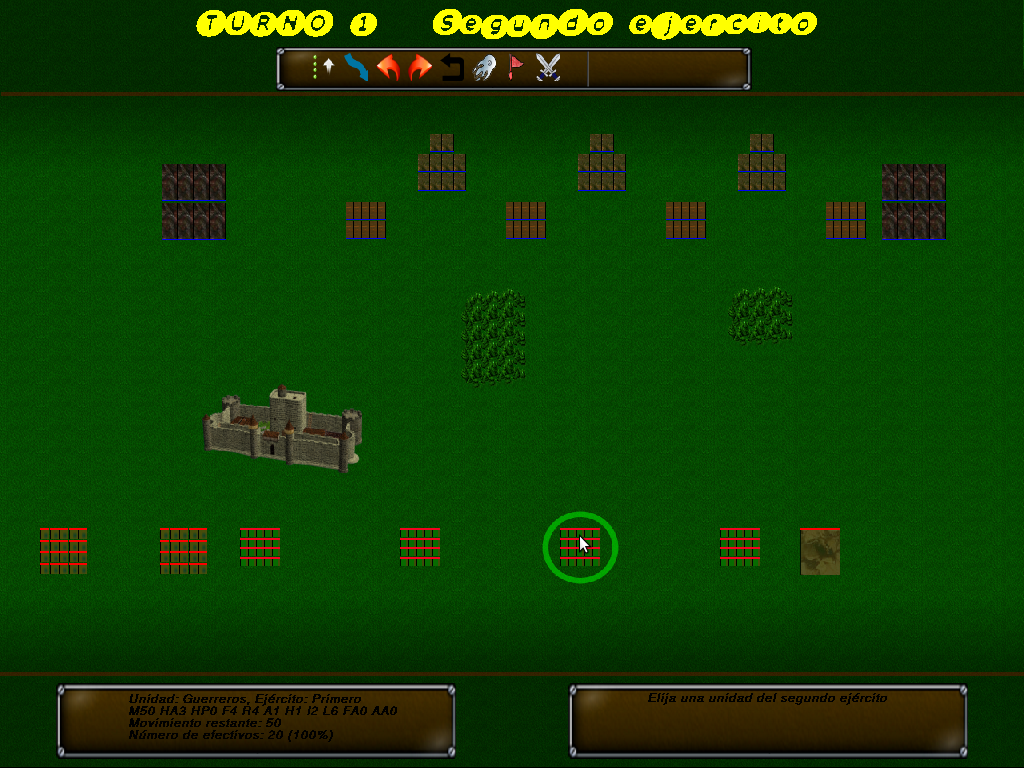
\includegraphics[scale=.4]{./imagenes/campobatalla.png}
\label{fig:campobatalla}
\caption{Campo de batalla}
\end{figure}

Cada una de éstas secciones de la pantalla de batalla se comentan a continuación.

\subsection*{Zona de iconos}
La zona de iconos reside en la parte superior del campo, en la zona
verde sombreada, justo encima de la franja roja transparente
superior.

Posee dos partes diferenciadas, el título de turno, y el menú de
iconos. El título de turno es sencillamente una descripción textual
del turno o situación actual: \textit{\textsc{Ejércitos desplegados}},
\textit{\textsc{Turno 1 Ejército primero}}, \textit{\textsc{Turno 1
    Ejército segundo}}, \textit{\textsc{Turno 2 Ejército primero}},
etc.

La zona de iconos es donde propiamente están todos los iconos que
permiten realizar todas las acciones del juego. Se diferencias dos
partes separadas por una barra, dentro del marco donde residen los
iconos.

En la primera parte, o parte izquierda, están todos los iconos que
pueden usarse ahora mismo para realizar acciones. Aparecen centrados
en su zona correspondiente. En la segunda, o parte derecha, aparecen
apiladas a la izquierda (como si de una secuencia se tratara), todos
los iconos que están activos pero no disponibles, esto es, de tareas
pendientes.

Si se pulsa en cualquiera de los iconos de la \textit{primera
  categoría}, se ejecuta su acción inmeditamente. Si se pulsa en
cualquiera de los iconos de la segunda, no se realiza ninguna acción
en el campo de batalla.

\subsection*{Zona de descripciones}
La zona de descripciones distingue dos partes, un primer marco, o
marco izquierdo, y un segundo marco, o marco derecho.

En el marco izquierdo, se muestra información de los elementos en los
que esté situado actualmente el ratón.

Si el ratón está situado en la zona de iconos, justo encima de alguno,
se muestra en este marco la descripción de la utilidad de dicho icono.

Si el ratón está situado encima de una unidad del campo de batalla, se
muestra, y en este orden:

\begin{itemize}
\item el nombre de la unidad.
\item el ejército al que pertenece a la unidad.
\item el perfil de atributos de la unidad.
\item la cantidad de movimiento restante de la unidad.
\item el número de efectivos actual de la unidad, junto al porcentaje
  de efectivos actuales respecto al original.
\item una descripción del estado especial de la unidad: huyendo,
  marchando o combatiendo. Si la unidad no está en ninguna de estas
  tres situaciones, no se mostrará nada acerca del estado de la unidad
  (su estado es el normal y predeterminado).
\end{itemize}

Si el usuario intenta realizar una acción no permitida, se muestra, en
el segundo panel, una breve descripción del motivo del error.

\subsection*{Campo de batalla}
El campo de batalla es el delimitado por arriba y por abajo por una
línea semitransparente de color rojo, que marca, junto con los bordes
de la pantalla, el límite del campo de batalla.

Dentro se sitúan todas las unidades presentes en la partida. Si una
unidad se retira de la batalla, su unidad no volverá a aparecer en el
campo de batalla.

La zona de despliegue del jugador uno es la parte inferior del campo
de batalla, y ocupa el primer 25\%, en dirección vertical, del campo
de batalla. La zona de despliegue del jugador dos es el 25\% superior
del campo de batalla.

\subsubsection*{Unidades}
Las unidades aparecerán como un conjunto homogeneo de efectivos, donde
cada efectivo es representado como un cuadrito con un dibujo
decorativo que distingue a los efectivos de una unidad de las
restantes. No existirán dos unidades distintas que tengan un igual
dibujo para sus efectivos.

A cada ejército le corresponderá un color. Al primero le corresponderá
el color rojo. Al segundo, el color azul. Los efectivos tienen
coloreado con el color de su equipo su propio frente, y además, cuando
se pasa el ratón por encima de una unidad, la circunferencia que
muestra la unidad apuntada por el ratón tendrá también el color de la
equipo de la unidad.

\subsubsection*{Escenografía}
El escenario posee un número aleatorio de elementos de escenografía
repartidos por el escenario, pero nunca en las zonas de despliegue ni
en sus cercanías.

En el reglamento de \gom se permite una total libertad a la hora de
tratar y colocar elementos de escenografía en el escenario.

En \gom se ha establecido la escenografía del juego de la siguiente
forma:
\begin{itemize}
\item Se divide el campo de batalla (excluyendo la zona de despliegue
  y el espacio de separación impuesto por el reglamento de \gomf) en 2
  ó 3 secciones. Esta cantidad se selecciona al azar.
\item De entre éstas 2 o 3 secciones, a una le corresponderá un
  edificio. A las restantes bosques.
\item La posición del edificio será determinada al azar dentro de su
  sección de campo correspondiente.
\item La posición de cada bosques también será determinada al azar
  dentro de su sección de campo correspondiente, así como el tamaño
  del mismo, que nunca corresponderá a un área mayor al 10\% de dicha
  sección.
\end{itemize}

Los elementos de escenografía, además, también imponen respetar un
espacio igual al espacio de unidades entre ellas, además de ser terreno impasable.

\subsubsection*{Transcurso de la batalla}
Al comenzar la batalla, las unidades aparecerán desplegadas en su
correspondiente lugar de acuerdo a la configuración del ejército
diseñado. A partir de entonces, los jugadores podrán, haciendo uso de
los iconos, y interactuando con el sistema, ejecutar todas las
acciones deseadas por el usuario, así como las requeridas por \gomf.

Una unidad siempre podrá seleccionarse con solo pulsar con el ratón
encima de ella. Al hacerlo, se mantenderá una circunferencia de color verde indicando que la unidad ha sido
seleccionada. Si se ejecuta alguna acción, y ésta se aplica a una
unidad (por ejemplo, un giro), la acción se ejecutará sobre esa
unidad. Si la acción se aplica a una unidad, y no hay ninguna
seleccionada, o hay seleccionada una del bando contrario al turno en
curso, se indica un mensaje de error en el marco derecho de la zona de
descripción..

Las acciones que necesiten información por parte del usuario son
pedidas dinámicamente en el campo de batalla. Por ejemplo, si una
unidad desea realizar un desplazamiento, se mostrará una zona
sombreada correspondiente al área dentro del cual la unidad podrá
desplazarse.

Apuntando con el ratón dentro de dicho área, se mostrará un cuadro
ficticio indicando la posición final de la unidad. Al pulsar sobre una
posición dentro del área, la unidad se mueve definitivamente a esa
posición.

Este comportamiento es igual en todas las acciones que
requieren información por parte del usuario, como el desplazamiento a
realizar, en el caso anterior. Se dispondrá de unos indicativos
visuales a las que el usuario deberá responder.

La batalla finaliza al llevar 6 turnos de juego, o al indicarlo el
usuario con el icono correspondiente.

\subsubsection*{Pantalla de resultado del combate}
Al finalizar la batalla, se muestra un menú que indica al ganador de
la batalla y la distribución en puntos de la misma.

Se divide en 4 partes:
\begin{itemize}
\item Descripción de los puntos del jugador 1.
\item Descripción de los puntos del jugador 2.
\item Sumario comparativo.
\item Ganador.
\end{itemize}

\begin{figure}[h]
\centering
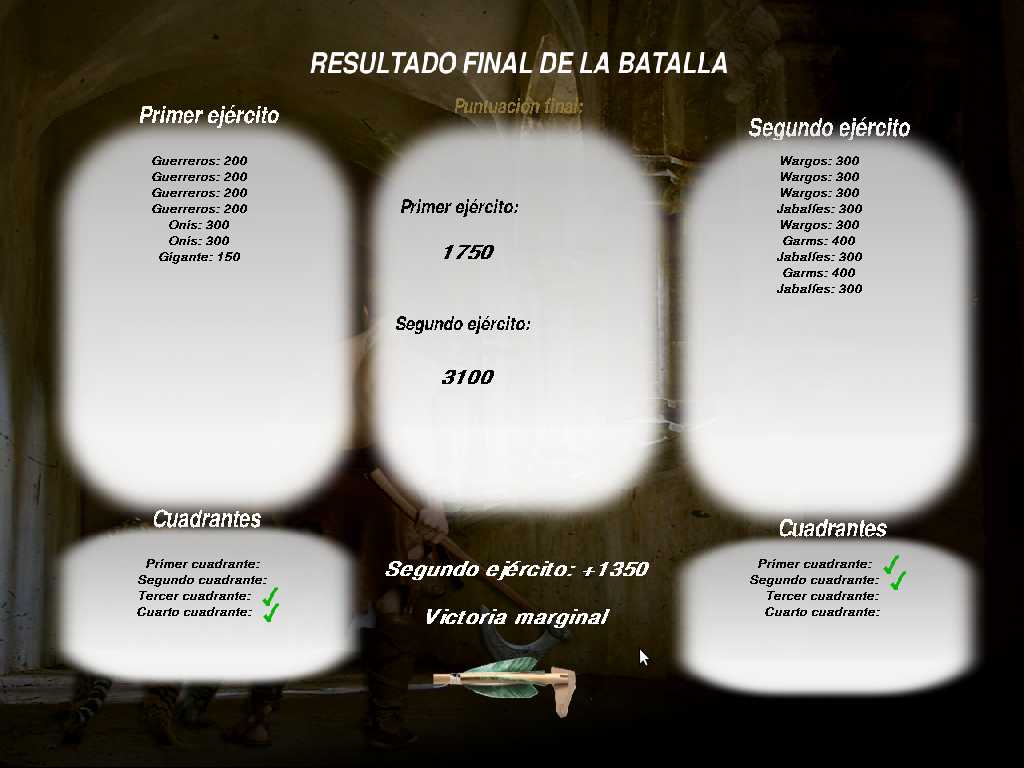
\includegraphics[scale=.4]{./imagenes/resultado.png}
\label{fig:imgresultado}
\caption{Menú de resultado de la batalla}
\end{figure}


\paragraph{Descripción de los puntos del jugador 1 y 2}
Son dos secciones que se encuentran, respectivamente, a la izquierda y
a la derecha de la pantalla para los jugadores 1 y 2. En ambos lados,
existe una parte superior que muestra las unidades, y una parte
inferior que muestra los cuadrantes.

En la descripción de las unidades, se coloca la puntuación obtenida
por ella tal y como expone el reglamento de \gom en su sección
correspondiente al resultado de una batalla.

En la descripción a los cuadrantes, se muestra una lista de cuatro
cuadrante y una señal de acierto para los cuadrantes que hayan caido
en posesión del ejército correspondiente.

\paragraph{Sumario comparativo}
Es la zona que está en el centro de este menú, la más alta. Se muestra
la ponderación total en puntos de ambas unidades, es decir, la suma de
los puntos obtenidos por unidades y por cuadrantes.

\paragraph{Ganador}
Se muestra el nombre del jugador ganador, así como el tipo de
victoria: \emph{masacre}, \emph{victoria decisiva} o \emph{victoria
  marginal}.

Si la partida acaba en \emph{empate}, evidentemente no habrá ningún
ejército ganador que mostrar y solo se indicará que la situación final
de la pantalla ha sido un empate.